\chapter{Conceptual and Mathematical Model}\label{chapter:conceptualmodel}
\thispagestyle{empty}

This chapter deals with the terms' definition and governing equations used in the model that was 
implemented in the numerical simulator \DuMuX. It also explains the mathematical model 
in implementing reactive source and sink terms in \DuMuX and \MATLAB. The conservation of mass and momentum equations, 
and the governing chemical kinetics in the implemented numerical method, together with the boundary 
and initial conditions that are necessary to solve the differential equations are explained in this chapter. 

\section{Introduction}
Mass transport occurs between a liquid phase i.e., CO\textsubscript{2}-enriched water and a solid phase 
i.e., calcite surfaces in caves as the dissolution advances where ionic species from the solid surface are 
released into the solution, and as precipitation where solid crystals are formed. The scope of our study 
is limited to modeling calcite dissolution in the cave surfaces. The conservation of a 
fluid quantity is the net effect of the transport of fluid across control volume boundaries by convection, 
diffusion, and sources/sinks within the control volume.
 
\section{Phases and components}
A phase is defined as the continuous region in space where the fluid properties such as density, viscosity, etc., are uniform. 
These phases may comprise several chemical components or just one chemical component mixing and forming a homogeneous region. 
The model discussed in this thesis has one phase i.e., the liquid phase, and three components i.e., \ce{H2O, CO2} and calcium.

\section{Continuity equation}
For each component i.e., $\kappa$ $\in$ \{ \ce{H2O, CO2}, calcium\}, the continuity equation/mass balance equation is defined as:
\begin{equation}\label{eq:contiEq} % Give a unique label
 \frac{\partial (\rho \mathrm{X}\textsuperscript{$\kappa$})}{\partial t} 
 + \nabla\cdot(\rho\textbf{v}\mathrm{X}\textsuperscript{$\kappa$} - \mathrm{D}\textsuperscript{$\kappa$}\rho\nabla 
 \mathrm{X}\textsuperscript{$\kappa$}) = \mathrm{Q} ,
\end{equation}
where:
\begin{itemize}
\item $\rho$, density of the fluid dependent on concentration of CO\textsubscript{2} and calcium, and other cave minerals [kg/m\textsuperscript{3}]
\item X\textsuperscript{$\kappa$}, mass fraction of each component i.e.,\{ \ce{H2O, CO2}, calcium\} [-]

\item \textbf{v} = [u, v, w]\textsuperscript{T}, the velocity vector [m/s]

\item D, binary diffusion coefficient [\ce{m^2}/s]

\item Q, source/sink term, which accounts for \ce{CO2} and calcium [kg/m\textsuperscript{3}s]\\
The term comes from the chemical reaction on the surface of the wall. It is defined and described in section \ref{sec:reactivesource}.

\end{itemize}
The density of water increases slightly with the dissolution of \ce{CO2} \cite{garcia2001density} and calcite 
\cite{zhao2015solubility}. Although the pressure we are interested in is fairly low (1 atm) compared to the pressures 
in \cref{fig:DensityH2OCO2}, we can imply that the density of \ce{H2O-CO2} system will increase as more \ce{CO2} is added into the karst water. \\
For the modeling purpose, we set the density of water to be the density of \ce{H2O-CO2-calcium} system as we did not consider 
the density change due to the addition of \ce{CO2} and calcium into the aqueous solution, making it less sophisticated and comparable 
with the \MATLAB results. We are interested in developing a 2D model of size 5mm $\times$ 15mm that implements calcite dissolution as a source/sink term, 
so the employed limitations will have negligible influence, if any, in altering the rate of dissolution and steady-state concentrations. \\

\begin{figure}
\centering
%for .eps, .png, etc use:
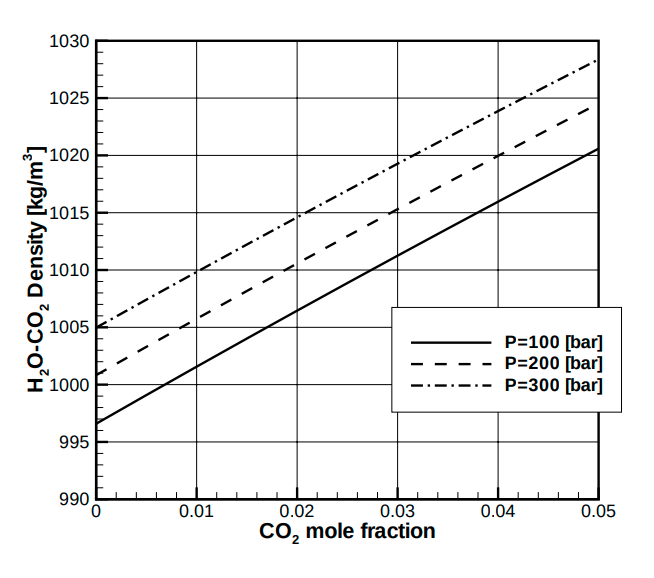
\includegraphics[width=0.6\textwidth]{PICTURES/H2O-CO2_Density.png}
%for tikz figures use:
%\input{your_file.tex}
\caption{Density variation of aqueous solution of \ce{CO2} \cite{garcia2001density}}
\label{fig:DensityH2OCO2}       % Give a unique label
\end{figure}

\section{Navier-Stokes equation}
The Navier-Stokes equations, which describe motion for Newtonian fluids, are formulated as: 
(A complete derivation can be found on \citet{white1979fluid}.)

\begin{equation}\label{eq:NSeq} % Give a unique label
 \frac{\partial (\rho \textbf{v})}{\partial t}
 + \nabla\cdotp (\rho \textbf{vv}\textsuperscript{T}) = \nabla\cdot(\mu(\nabla\textbf{v} + \nabla\textbf{v}\textsuperscript{T})) - 
 \nabla \mathrm{p} + \rho \textbf{g},
\end{equation}

where:
\begin{itemize}
\item $\mu$, Dynamic viscosity of the fluid [\ce{m^2}/s]
\item p, pressure [kg/m\ce{s^2}]
\item \textbf{g}, gravity vector [m/\ce{s^2}]
\end{itemize}

We assume incompressibility of the fluid. Hence, Navier-Stokes equation results in:
\begin{equation}\label{eq:NSeqincompress} % Give a unique label
 \frac{\partial ( \textbf{v})}{\partial t}
 + \nabla\cdotp (\textbf{vv}\textsuperscript{T}) = \nu\nabla\cdot(\nabla\textbf{v} + \nabla\textbf{v}\textsuperscript{T}) - 
 \nabla \mathrm{w} + \textbf{g},
\end{equation}
where:
\begin{itemize}
    \item $\nabla \mathrm{w} = \frac{1}{\rho_0}\nabla \mathrm{p}$ [\ce{m^2}/\ce{s^2}],
    \item $ \nu = \frac{\mu}{\rho_0}$ is called as kinematic viscosity [\ce{m^2}/s].
\end{itemize}


\section{Boundary and initial conditions}
To obtain a unique solution of the governing equations, initial and boundary conditions must be specified. \\
The initial conditions of the primary variables must be specified throughout the computational domain \textit {V}. 

\begin{equation}\label{eq:initCondition} % Give a unique label
 \phi(\textbf{r},t_0) = \phi^0(\textbf{r}), \quad \textbf{r} \in \textit{V}.
\end{equation}

Boundary conditions must also be specified around the computational domain, \textit{S}\textsubscript{B}, throughout 
the simulation time. Based on the nature of the boundary value, boundary conditions are categorized as follows: 
\begin{itemize}
    \item \textbf{Dirichlet} boundary condition \quad The value of the dependent variables on the portion of the 
    boundary,$\textit{S}^{\textrm{D}}_{\textrm{B}}$ is known.
    
    \begin{equation}\label{eq:dirichletCondition} % Give a unique label
        \phi(\textbf{r}_B,t) = f(t), \quad \textbf{r}_B \in \textit{S}^{\textrm{D}}_{\textrm{B}}.
    \end{equation}
    
    On solid walls, Dirichlet condition for velocities is imposed (no-slip condition).
    
    \item \textbf{Neumann} boundary condition \quad The gradient of the dependent variables on the portion of the 
    boundary, $\textit{S}^{\textrm{N}}_{\textrm{B}}$, is known.
    
    \begin{equation}\label{eq:neumannCondition} % Give a unique label
        \textrm{grad } \phi (\textbf{r}_B,t) = f(t), \quad \textbf{r}_B \in \textit{S}^{\textrm{N}}_{\textrm{B}}.
    \end{equation}
    
    \item \textbf{Outflow} boundary condition \quad Outflow boundary conditions are assigned where the flow is almost 
    unidirectional and the surface stresses/pressure are known \cite{versteeg2007introduction}.
    \begin{equation}\label{eq:outflow}
        \mathrm{grad}(\phi)*\mathrm{n} = 0, \quad \ce{p} = \ce{p_{ext}},
    \end{equation}
    where, $\phi$ is a variable (e.g. mass fraction of \ce{CO2}: X\textsuperscript{$\wedge$}\ce{CO2}), n is a unit vector 
    normal to the boundary and \ce{p_{ext}} is the external pressure/pressure at the boundary.\\
    
    \item \textbf{Symmetric} property \quad It is useful to take advantage of symmetries in the flow field when the model 
    is symmetric with respect to its orientation and boundary conditions. 
    We can impose the following symmetric properties along the center of the domain and only solve half of it.
    \begin{equation}\label{eq:symmetric}
        \nabla p\cdot \mathbf{n} = 0, \quad \nabla v_t \cdot \mathbf{n} = 0, \quad v_n = 0,
    \end{equation}
    where $v_t$, $v_n$ are the tangential and normal components of the velocity.
    
\end{itemize}
The implementation of boundary conditions is presented in \cref{chapter:modelconcept}.

\section{Reactive source and sink terms}\label{sec:reactivesource} The source and sink terms account for total inorganic carbon 
(\ce{CO2}, \ce{H2CO3}, \ce{CO3^{2-}}, and \ce{HCO3^{-}}) and calcium. 
There could be several other cave minerals, but the scope of this thesis is limited to calcite. \\
We assumed abundant calcite in our model -- and for an opened system (see \cref{chapter:modelconcept}) 
the base-flow is further carrying the dissolved calcite out of the domain -- so that the aqueous phase is always under-saturated with 
calcium in both opened (with a base-flow) and closed (without a base-flow) systems. Therefore, we neglect the precipitation rate. 
The rate of calcite dissolution determines the source terms calcium ($\ce{q^{Ca}}$), and total inorganic carbon (\ce{q^{TIC}}).

\begin{equation}\label{CalciumDiss}
\ce{q^{Ca}} = \ce{r_{diss}},
\end{equation}

\begin{equation}\label{CalciteDiss}
\ce{q^{TIC}} = \ce{r_{diss}},
\end{equation}

where: \ce{r_{diss}} [mol/\ce{m^3}s] is the rate of calcite dissolution. For a 2D domain, the unit is [mol/\ce{m^2}s].\\

 The dissolution rate of calcite:
\begin{equation}\label{eq:rDiss}
\ce{r_{diss}} = \left(\ce{k_{diss,1}}\ce{m^{\ce{H^{+}}}} + \ce{k_{diss},2}\right)\ce{A_{cw}}(\Omega - 1)^{\ce{n_{diss}}}; 
\quad \textrm{for } \Omega < 1,
\end{equation}
and,

\begin{equation}\label{eq:omega}
\Omega = \frac{\ce{m^{Ca^{2+}}}\gamma^{\ce{Ca^{2+}}}\ce{m^{CO_3^{2-}}}\gamma^{\ce{CO_3^{2-}}}}{\ce{K_{sp}}},
\end{equation}

where: 

\begin{itemize}
\item \ce{m^{\ce{H^{+}}}}: molality of hydrogen ion [\ce{mol_{\ce{H^+}}}/\ce{kg_{\ce{H2O}}}].\\
\item \ce{A_{cw}} is specific area which is the ratio of inter-facial area where dissolution occurs in a cell to the volume of 
the cell [\ce{m^2}/\ce{m^3}]. For a 2D domain, the unit is [\ce{m^2}/\ce{m^2}]. \\
\item \ce{m^{\ce{Ca^{2+}}}} and \ce{m^{\ce{CO3^{2-}}}}: the molalities of calcium [\ce{mol_{\ce{Ca^{2+}}}}/\ce{kg_{\ce{H2O}}}] 
and carbonate [\ce{mol_{\ce{CO3^{2-}}}}/\ce{kg_{\ce{H2O}}}] respectively. \\
\item \ce{$\gamma^{CO_3^{2-}}$} and \ce{$\gamma^{Ca^{2+}}$}: component activities (we assumed 1.0) [-].\\
\item \ce{k_{diss,1}}, \ce{k_{diss,2}} and \ce{n_{diss}} are dissolution constants \cite{chou1989comparative}, \cite{compton1989dissolution}. \\
\begin{itemize}
    \item \ce{k_{diss,1}} = $10^{-6.352}$ [\ce{mol_{\ce{Ca^{2+}}}/\ce{m^2s}}]/[\ce{mol_{H}}/\ce{kg_{\ce{H2O}}}]\\
    \item \ce{k_{diss,2}} = $10^{-10.329}$ [\ce{mol_{\ce{Ca^{2+}}}}/\ce{m^2}s]\\
    \item \ce{n_{diss}} = 1 [-] \\
\end{itemize}
\item \ce{K_{sp}}: calcite solubility product.\\
\begin{itemize}
    \item \ce{K_{sp}} = $10^{-8.48}$ [\ce{mol^2/kg^2_{\ce{H2O}}}]\\
\end{itemize}
\end{itemize}




\paragraph*{Dissociation reaction and change in pH}\mbox{}\\ \\
Dissolution of calcite produces \ce{Ca^{2+}}, \ce{CO_3^{2-}}, \ce{HCO_3^{-}}, \ce{H^+}, and \ce{OH^-} in the solution. 
The rate of dissolution of calcite depends on molality of hydrogen ion (\ce{m^{H+}})/pH, calcium (\ce{m^{\ce{Ca^{2+}}}}) and 
carbonate (\ce{m^{\ce{CO3^{2-}}}}) see \cref{eq:rDiss,eq:omega}, but carbonate depends on total inorganic carbon (TIC) and 
molality of hydrogen ion, \cref{fig:dissKinetics}. At the beginning, when there is no calcium in the solution, the rate of dissolution is at the highest. 
Carbonic-acid is the fuel for calcite dissolution, and it's being used up during dissolution. 
If the used-up carbonic-acid is not replenished, calcite dissolution comes to naught after carbonic-acid ceases to exist in the solution. 
Such is the case with closed-systems where the initial dissolution potential is never replenished. In an opened-system, though, replenishment of 
carbonic-acid occurs as the fingers of \ce{CO2} protruding into the karst water enriches the water with carbonic-acid. Hence, there is a constant 
rate of dissolution at the steady-state in an opened-system. Steady-state depends on several factors such as flow-velocity -- if it's an opened 
system -- initial pH and TIC of the solution, and amount of \ce{CO2} above the epiphreatic karst water table -- if it's an opened system -- which will be 
discussed in  the subsequent chapters. \\

\begin{figure}
\centering
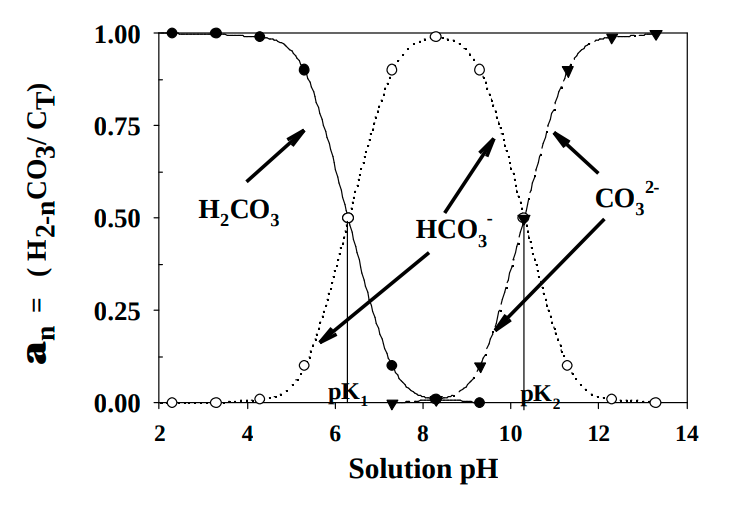
\includegraphics[width=0.7\textwidth]{PICTURES/dissolutionKinetics.png}
\caption{The distribution of carbonate species as a fraction of total dissolved carbonate vs pH \cite{butler1991carbon}}
\label{fig:dissKinetics}
\end{figure}

The law of mass action for the dissociation of water is used to calculate the activity of \ce{H^+}.
\begin{equation}
[\ce{H^+}][\ce{OH^-}] = \ce{K_w},
\end{equation}

where: \ce{K_w} = $10^{-14}$ is the dissociation constant and [\ce{H^+}] and [\ce{OH^-}] are the activities of \ce{H^+} and \ce{OH^-} 
respectively. The charge balance states:
\begin{equation}
\sum\limits_{i=1}^{\textrm{charged components}} \ce{z^i}\ce{m^i} = 0,
\end{equation}
where: \ce{z^i} is the charged component i and \ce{m^i} is its molality. The resulting charge balance equation for the dissolution 
of calcite can be expanded as:
\begin{equation} \label{eq:chargebal}
2\ce{m^{Ca^{2+}}} - 2\ce{m^{CO_3^{2-}}} - \ce{m^{HCO_3^-}} + \ce{m^{\ce{H^{+}}}} - \ce{m^{\ce{OH^{-}}}} + \ce{mCorrection} = 0,
\end{equation}

where,
\[
\ce{m^{CO_3^{2-}}} = \frac{\ce{m^{TIC}}}{\frac{\left(\ce{m^{\ce{H^{+}}}}\right)^2}{\ce{k_{diss,1}} \cdot 
\ce{k_{diss,2}}}+1+\frac{\ce{m^{\ce{H^{+}}}}}{\ce{k_{diss,2}}}},
\]
and,
\[
\ce{m^{HCO_3^-}} = \frac{\ce{m^{TIC}}}{\frac{\ce{m^{\ce{H^{+}}}}}{\ce{k_{diss,1}}}+1+\frac{\ce{k_{diss,2}}}
{\ce{m^{\ce{H^{+}}}}}},
\]

Solving Eq. \ref{eq:chargebal} we get

\begin{equation} \label{eq:chargebalfinal}
2\ce{m^{Ca^{2+}}} - \frac{2\ce{m^{TIC}}}{\frac{\left(\ce{m^{\ce{H^{+}}}}\right)^2}{\ce{k_{diss,1}} \cdot 
\ce{k_{diss,2}}}+1+\frac{\ce{m^{\ce{H^{+}}}}}{\ce{k_{diss,2}}}} - \frac{\ce{m^{TIC}}}{\frac{\ce{m^{\ce{H^{+}}}}}
{\ce{k_{diss,1}}}+1+\frac{\ce{k_{diss,2}}}{\ce{m^{\ce{H^{+}}}}}} + \ce{m^{\ce{H^{+}}}} - \frac{\ce{K_w}}{\ce{m^{\ce{H^{+}}}}} + 
\ce{mCorrection} = 0,
\end{equation}

where mCorrection accounts for the initial charges in the system before the simulation/dissolution of calcite, 
due to the buffering capacity of water. It is calculated once at the beginning and added to the charge balance equation. 
\begin{equation}\label{eq:mCorrection}
\ce{mCorrection} = -2\ce{m^{Ca^{2+}}} + \frac{2\ce{m^{TIC}}}{\frac{\left(\ce{m^{\ce{H^{+}}}}\right)^2}{\ce{k_{diss,1}} 
\cdot \ce{k_{diss,2}}}+\frac{\ce{m^{\ce{H^{+}}}}}{\ce{k_{diss,2}}} + 1} + \frac{\ce{m^{TIC}}}{\frac{\ce{m^{\ce{H^{+}}}}}
{\ce{k_{diss,1}}} + 1 + \frac{\ce{k_{diss,2}}}{\ce{m^{\ce{H^{+}}}}}} - \ce{m^{\ce{H^{+}}}} + \frac{\ce{K_w}}{\ce{m^{\ce{H^{+}}}}}.
\end{equation}

\section{Compositional quantities and definitions}
This section defines a few terms used in the model formulation and implementation. 

\paragraph*{Mass fraction \& Mole fraction} Mass or mole fractions define the amount of components in a given phase. 
$\ce{x}_\alpha^\kappa$ is mole fraction of the component $\kappa$ in phase $\alpha$ and is defined as:

\begin{equation}\label{eq:moleFrac}
    \mathrm{x}_\alpha^\kappa = \frac{\mathrm{n}_\alpha^\kappa}{\sum_{i} \mathrm{n}_\alpha^i},
\end{equation}

$\ce{n}_\alpha^\kappa$ defines number of moles of component $\kappa$ in phase $\alpha$.
Similarly, mass fraction, $\ce{X}_\alpha^\kappa$, is defined as mass fraction of component $\kappa$ in phase $\alpha$, 
$\ce{X}_\alpha^\kappa$ = $\textrm{mass}_\alpha^\kappa/\textrm{mass}_\alpha^\textrm{total}$.
We used mass/mole-fraction while solving continuity equation \cref{eq:contiEq} for each component i.e., \ce{H2O, CO2, calcium}.

\paragraph*{Molality} The molality, $\ce{m}^\kappa$, is defined as the ratio of number of moles of component $\kappa$ in 
aqueous phase to the mass of pure water in aqueous phase.
\begin{equation}\label{eq:molality}
    \ce{m}^\kappa = \frac{{\ce{n}_{\textrm{aq}}}^\kappa}{\textrm{mass}_{\textrm{H}_\textrm{2}\textrm{O}}},
\end{equation}

Molalities are used in the chemical calculations because density effects at higher solute concentrations prohibit the use 
of concentrations, which depend on the volume. Likewise, the mole fractions of an inert component might change significantly 
during reactions, see \cref{eq:moleFrac} \cite{hommel2016modeling}. The mass of solvent on the other hand is more or less 
constant and consequently, $m^\kappa$ also has minor fluctuations, so we used molality while solving charge balance equation 
\ref{eq:chargebalfinal} to model calcite dissolution.

% \paragraph*{Henry's Law} Henry's Law is used to calculate amount of dissolved gas in a liquid based on the partial pressure of the gas above the liquid by assuming equilibrium between fluid phases. \\
% The implemented model uses Henry's law to calculate the amount of CO\textsubscript{2} dissolved in water based on the partial pressure of the CO\textsubscript{2} above it. According to Henry's law, mole fraction of CO\textsubscript{2}, $x^{\textrm{CO}_\textrm{2}}$ is:
% \begin{equation}\label{eq:henryLaw}
%     x^{\textrm{CO}_\textrm{2}} = H_{aq,\textrm{CO}_\textrm{2}}p_{\textrm{CO}_\textrm{2}},
% \end{equation}
% where,\\
% $H_{aq,\textrm{CO}_\textrm{2}}$ (in mol CO\textsubscript{2}/mol H\textsubscript{2}O.atm) is the Henry's constant, 
% $p_{\textrm{CO}_\textrm{2}}$ is partial pressure of $\textrm{CO}_\textrm{2}$.  

\endinput